\chapter{Project Design}

\section{System Requirement} % (fold)
\label{sec:system_requirement}

\begin{itemize}
\item Operating System: iOS 6
\item Compile with Automatic Reference Counting (ARC)
\item Hardware Used: iPhone 5 and iPod Touch 4th Generation
\end{itemize}
 
% section system_requirement (end)
\newpage

\section{Design Philosophy} % (fold)
\label{sec:design_pholosiphy}

\subsection{Singleton Design Pattern} % (fold)
\label{sub:singleton_design_pattern}

	Design Pattern is used in this project. In software engineering, the Singleton Pattern arms at creating the instance of a class only one time so that we don't need to create twice. It is especially useful when you need to use a method of the class while the class is just a toolkit for you. In this project, we could this pattern to create a Settings instance in order to keep Settings globally shared inside of the app. There are a bunch of other places use this pattern as well, such as NearbyVenueController, LocationManager etc. \\
	
% subsection singleton_design_pattern (end)

\subsection{Model-View-Controller} % (fold)
\label{sub:model_view_controller}

	Another popular design philosophy in software engineering field is Model-View-Controller. This separate each parts so that we could focus on one thing instead of all together. We could call it as a divide and conquer method. The benefit to use it is that if we changed one Controller function, sometimes we don't need to update the view for it. It is a time and life saver for app designing. \\
	
% subsection model_view_controller (end)
\newpage
\section{Architecture} % (fold)
\label{sec:architecture}

	Figure~\ref{fig:storyboard} shows main views in storyboard. In this project, we build it as a tab based application. Five tabs are created for different purpose. Home tab plays as a guide to create a foodie event; Foodie list tab shows all the events created before; Statistics tab shows all aggregated data; Searching tab is used to show all past events and searching by address to find the events locations; Setting tab is for configurations.
	
\begin{figure}
	\centering
    \SetFigLayout[5]{1}{1}
    {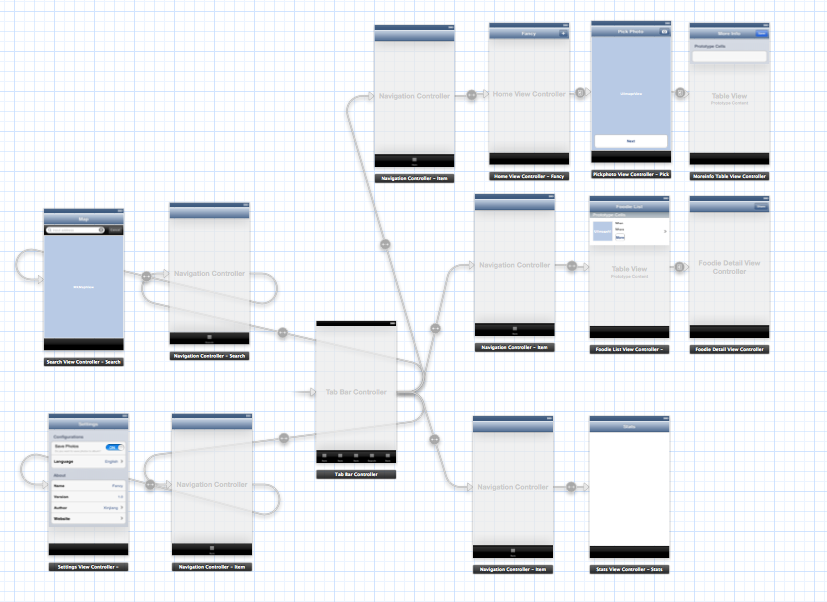
\includegraphics[%
    width=\figwidth, totalheight=\figheight, keepaspectratio]{./screenshots/storyboard-full.png}}
    \caption{Storyboard of Fancy Foodie}
	\label{fig:storyboard}
\end{figure}
% section architecture (end)
% section design_pholosiphy (end)



